%! TEX root = ./master.tex

\lecture{18}{Week 9}{Cache Optimisation}

Knowing the cache hierarchy is extremely important to write optimized code.

\paragraph{Problem}
CPU performance increased much faster than memory. This has lead to a gap which got greater over time. The solution to this problem are caches.

\paragraph{General Concept}
When we need some data, e.g. block b in the CPU, it it first checked, if the block is in cache. If it is not, the block is fetched from memory and placed in cache according to some placement policies. The next time the CPU needs block b, it can get it directly from cache.

\paragraph{Performance Metrics}
The three fundamental metrics are:

\begin{description}
    \item[Miss Rate:] Fraction of misses and total memory reference: $\text{misses} / \text{accesses} = 1 - \text{ hit rate}$.
        \begin{itemize}
            \item It tells how often to be have to go down the hierarchy to memory.
            \item Typically, it is $3-10$\% for L1 and $< 1$\% L2.
        \end{itemize}
    \item[Hit Time:] The time it takes to deliver a hit from the cache to the CPU, including the time required to determine of the data is in the cache.
        \begin{itemize}
            \item It is the time he have to stall in ordre to wait for data.
            \item Typically, it is $1 - 2$ clock cycles for L1 and $5 - 20$ clock cycles for L2.
        \end{itemize}
    \item[Miss Penality:] Additional time required on a miss to get the data from memory.
        \begin{itemize}
            \item Typically, $50 - 200$ clock cycles.
        \end{itemize}
\end{description}

The more we increase clock speed, the higher the time penalties get in cycles. This is the general trend.

Often, we use the miss rate when talking about cache access instead of hit rate. This is because the hit rate is sometimes a bit misleading. For a cache with hit time of $1$ cycle and miss penalty of $100$ cycles, we get an average hit time when assuming hit rates of $99$\% and $97$\% off:
\begin{itemize}
    \item $99$\% hits: $1 \text{ cycle } + 0.01 \cdot 100 \text{ cycles } = 2 \text{ cycles}$
    \item $97$\% hits: $1 \text{ cycle } + 0.03 \cdot 100 \text{ cycles } = 4 \text{ cycles}$
\end{itemize}

As we can see, a hit rate of $99$\% is twice as good as a hit rate of $97$\%.

\paragraph{Calculate Average Memory Access Time}
The following principle can be extended to $n$ level of caches:

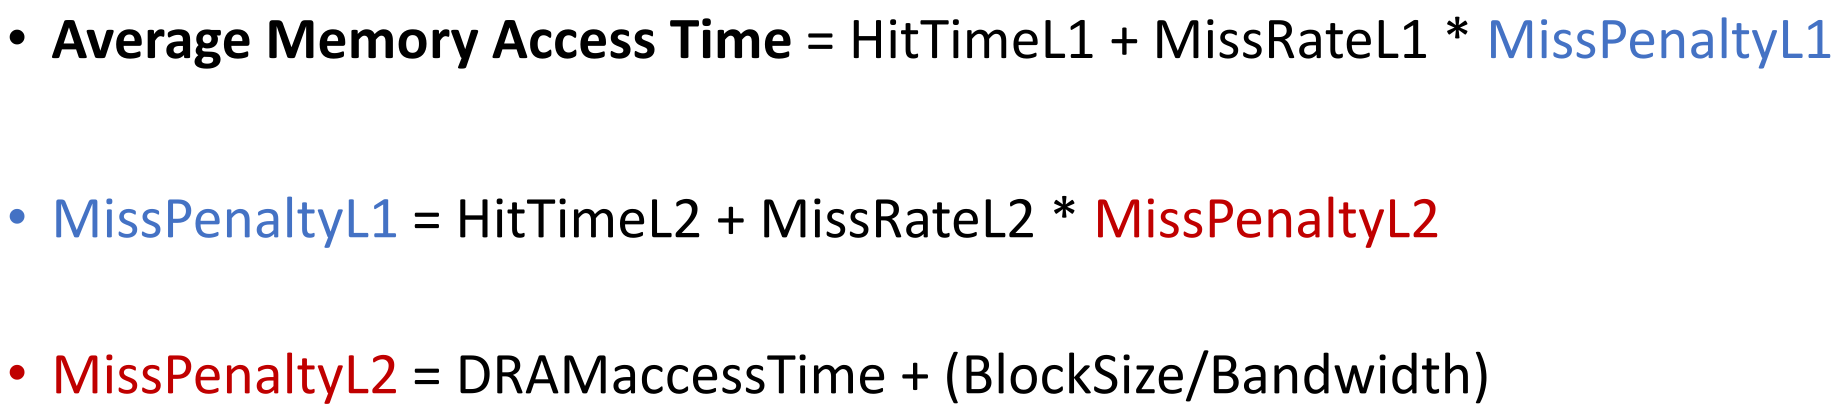
\includegraphics[width=1\textwidth]{18_cachePerformanceFormula.png}

\paragraph{Types of Cache Miss}
There are three main types of cache misses:

\begin{description}
    \item[Cold:] Occurs when the cache is empty and we access the first block
    \item[Conflict:] When at the designated location in the cache is a block, but not the one we are looking for
    \item[Capacity:] When the set of active cache blocks is larger than than the cache
\end{description}
Additionally, for muliprocessor systems, there is a fourth type, the \textbf{Coherency}. We will learn more about that later.

\subsubsection{Cache Organisation}

There are three parameters to describe the organisation of the cache.

\begin{description}
    \item[S] $= 2^s$ sets
    \item[E] $= 2^e$ lines per set
    \item[B] $= 2^b$ bytes per cache block (for data)
\end{description}

\begin{description}
    \item[Set:] Different part of the memory address map to different parts of the cache. A Set is one such part of the memory.
    \item[Entry/Way/Line:] Are the block in a set. When a cache is $n$-way, then $n$ different blocks can be held in one set.
\end{description}

Each block has:

\begin{description}
    \item[Valid Bit:] If set, the entry is actual a valid block.
    \item[Tag:] Helps to match the entry and determine of we have a hit.
    \item[Data:] The data of the block.
\end{description}

The cache has size $S \cdot E \cdot B$ bytes.

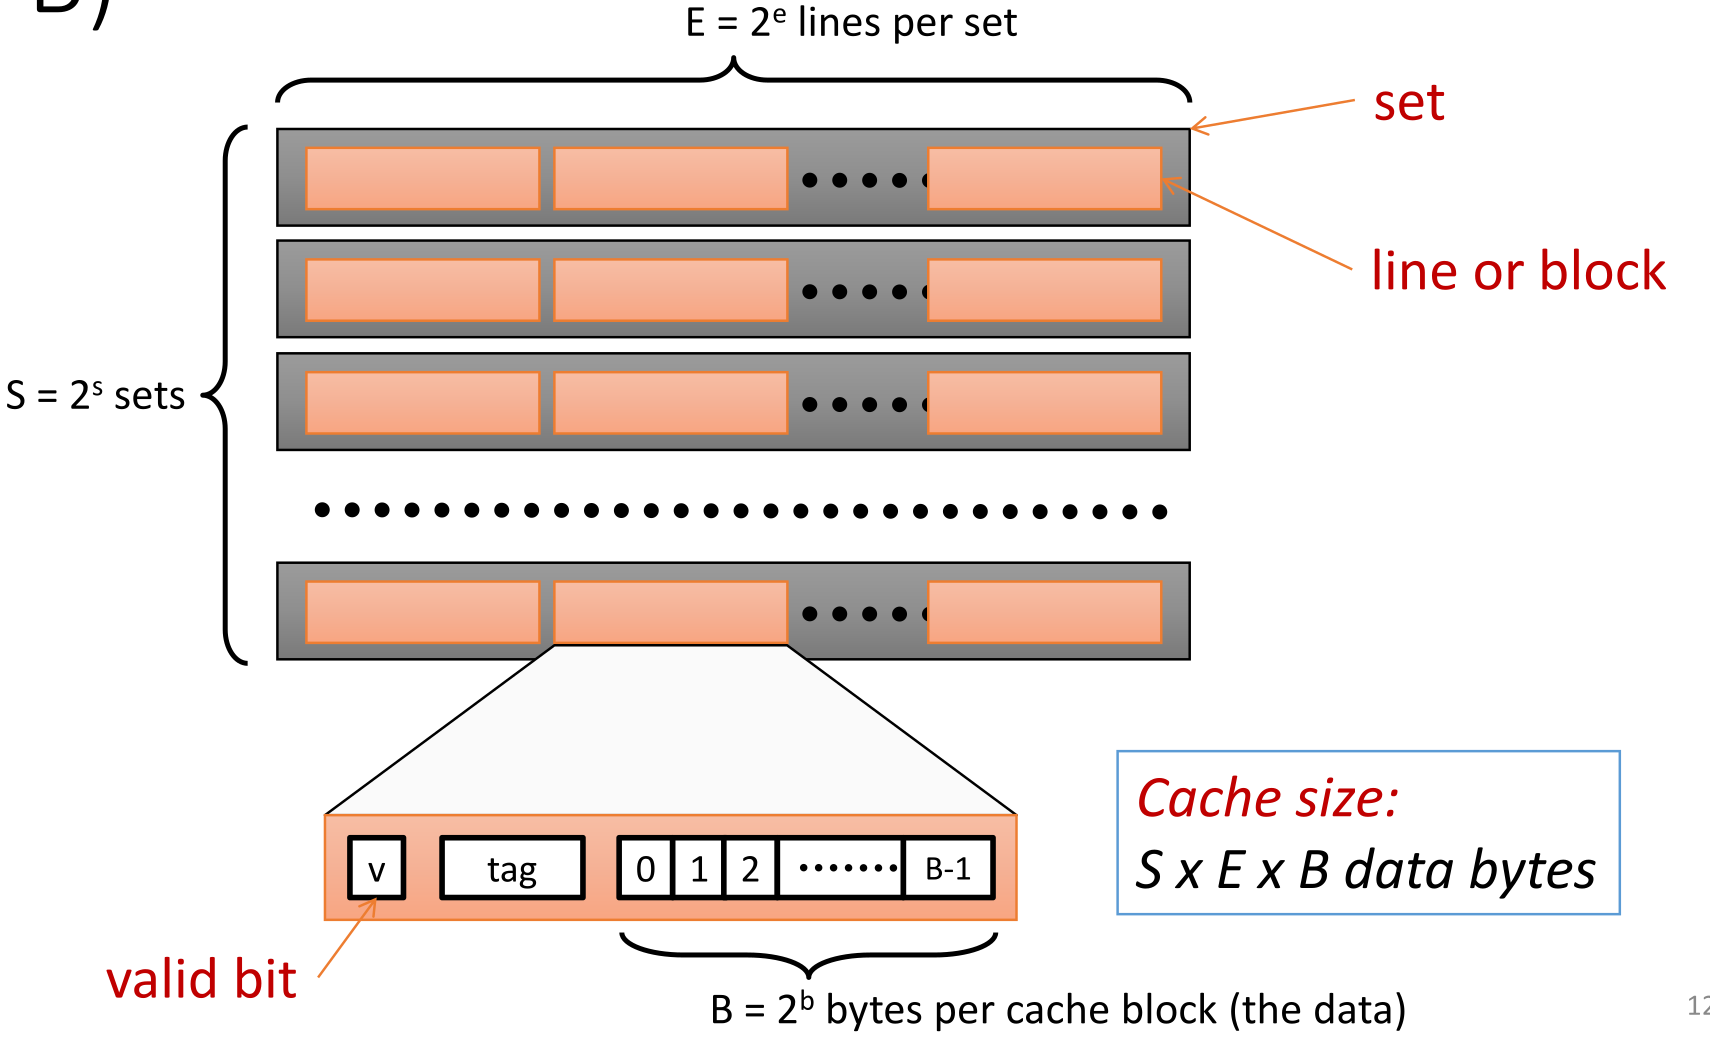
\includegraphics[width=1\textwidth]{18_cacheStructure.png}

\subsubsection{Cache Reads}
Given a memory address: In order to check if the desired block is already in memory, the address is split into three parts

\begin{description}
    \item[Block Offset:] Last $b$ bits.
    \item[Set Index:] The middle $s$s bits.
    \item[Tag:] The most important $t$ bits.
\end{description}

In order to check if the block is in cache, we proceed as follows:

\begin{enumerate}
    \item Locate the set using the set idex
    \item Check if any line/entry has a matching tag
    \item If yes and entry valid, we have a hit and the data starts at the offset
\end{enumerate}

Unlike memory, a cache block is not byte accessible, therefore we use a block offset in order to access the desired data.

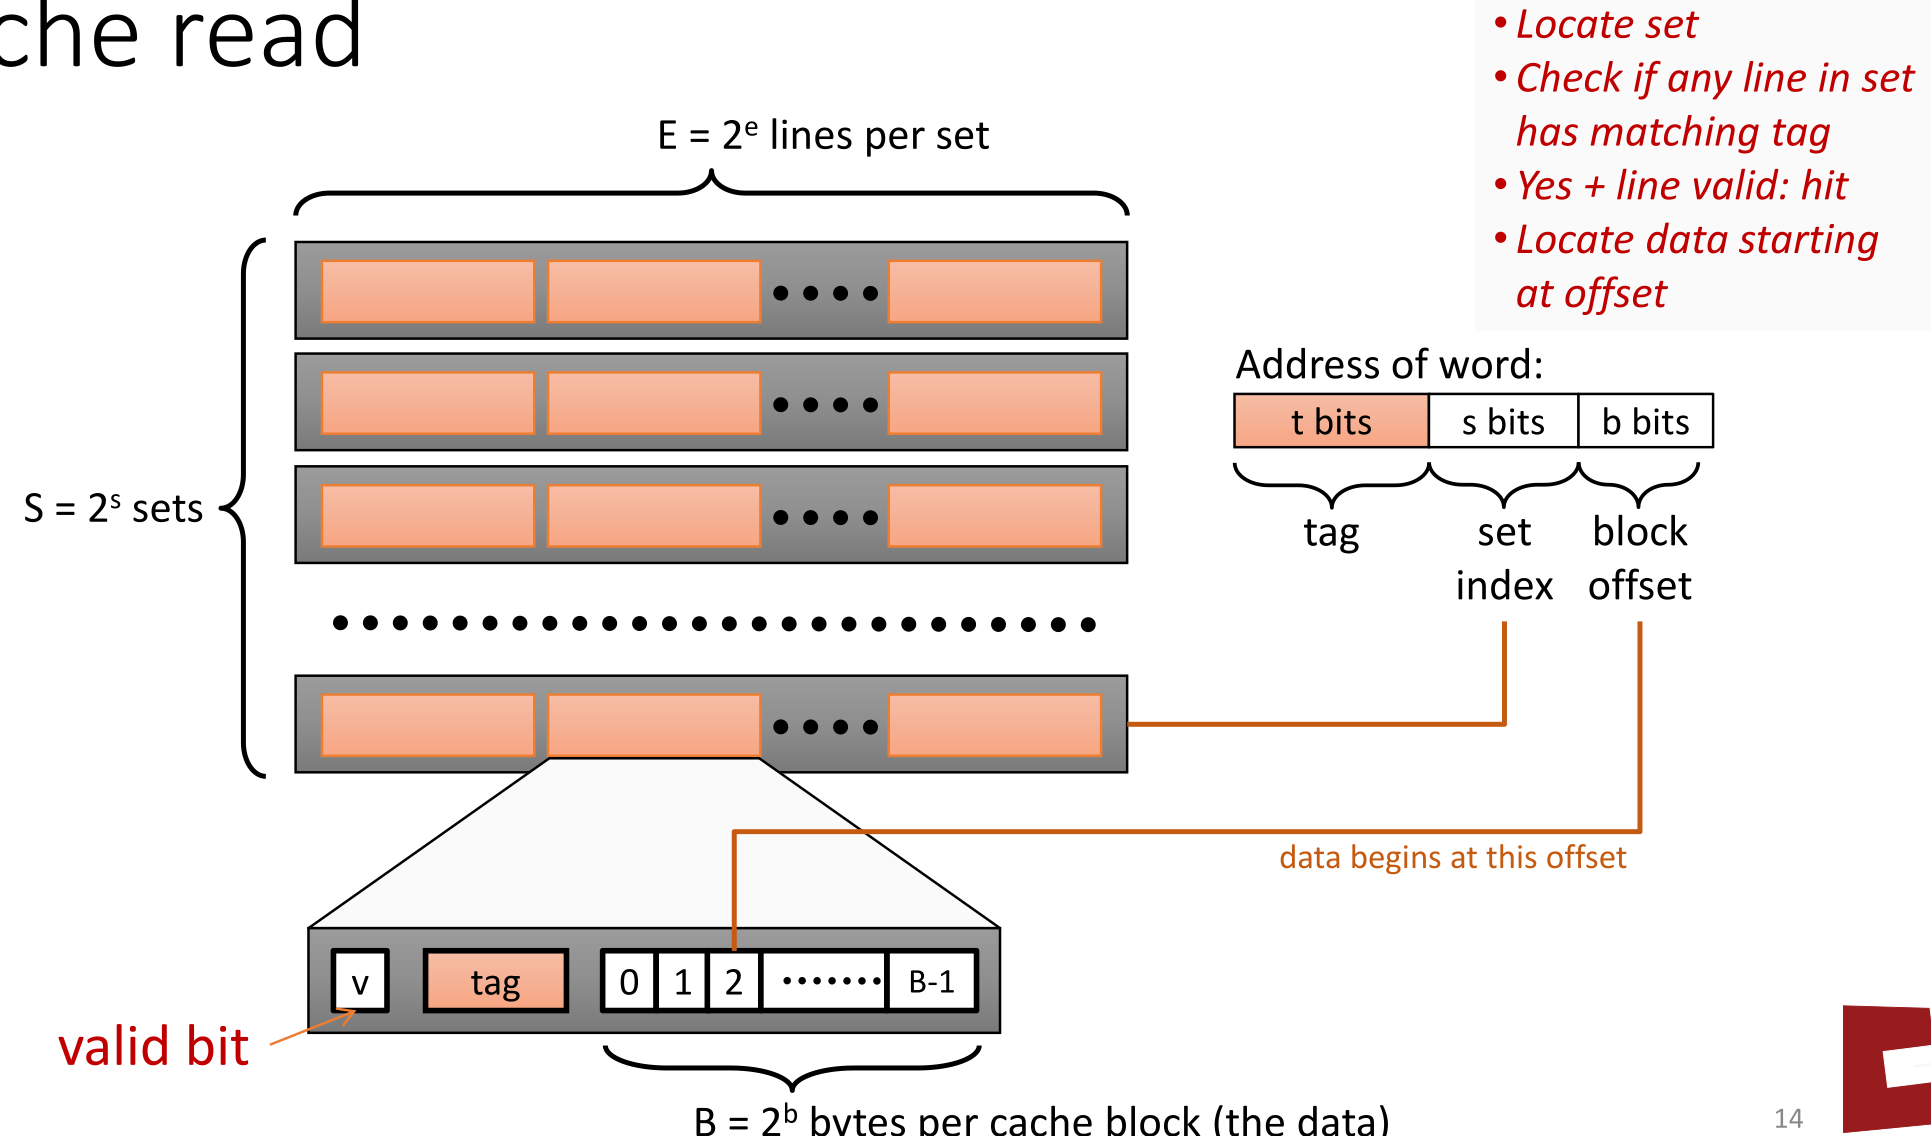
\includegraphics[width=1\textwidth]{18_cacheRead.png}

\paragraph{Types of Cache}
Caches different in their way. The simplest one is the $1$-way cache, called direct mapped cache.

\subparagraph{Direct Mapped Cache ($E=1$)}
This is the simplest type and each set contains only one entry.

The following image shows an example with a cache block of size $8$.

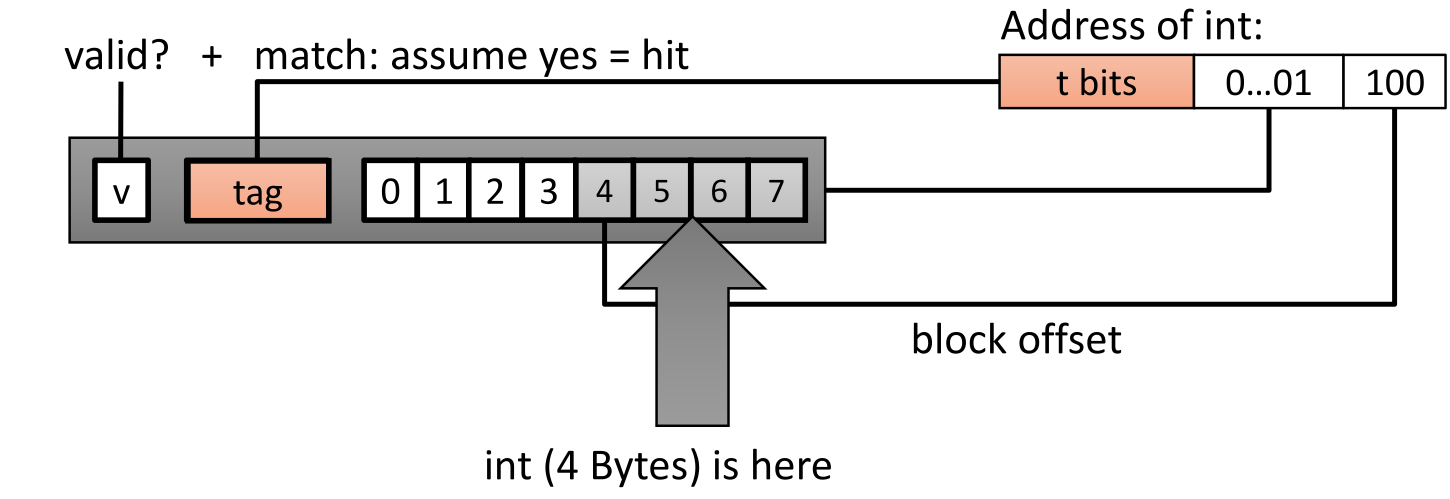
\includegraphics[width=0.8\textwidth]{18_directMapped.png}

If there is no match, the block is replaced by the newly fetched block.

\subparagraph{$2$-way Set-Associative Cache ($E=2$)}
Each set contains two lines. Again, we assume a cache block size of $8$ in the following example

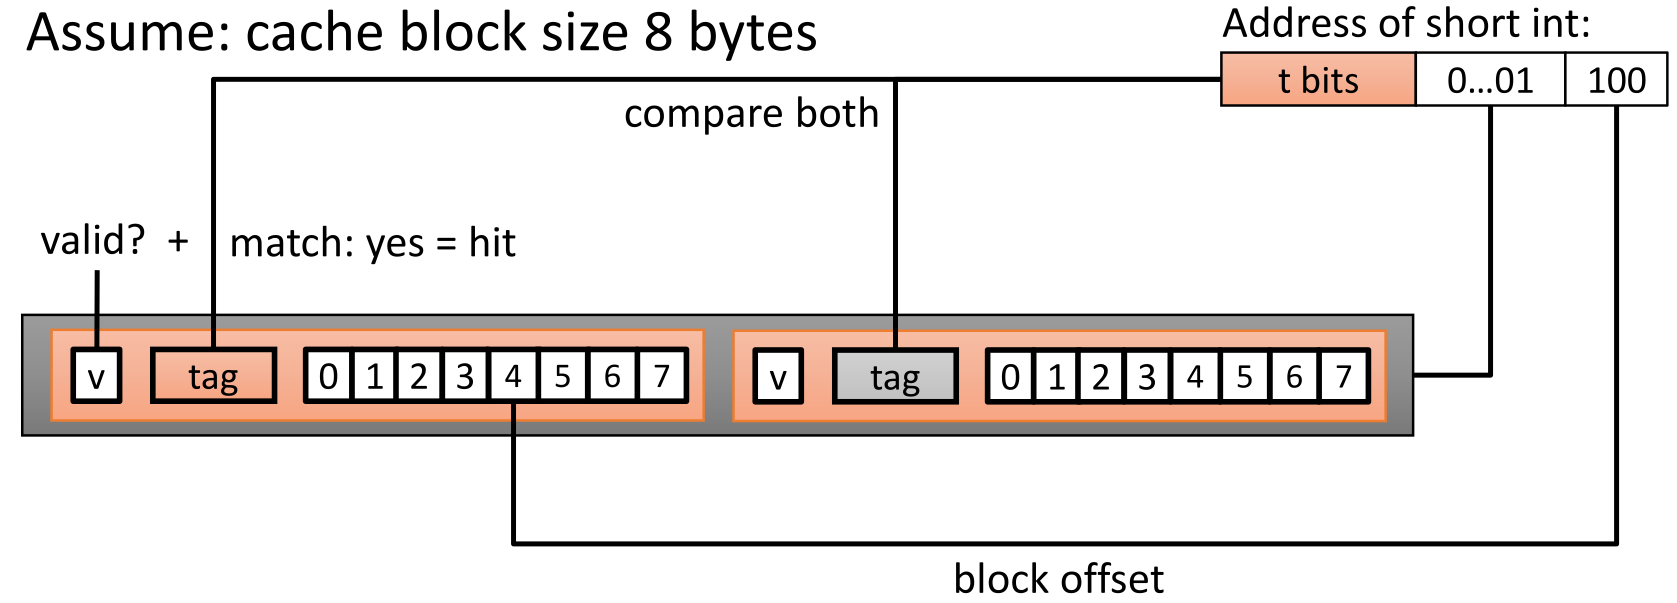
\includegraphics[width=0.8\textwidth]{18_2wayAssoc.png}

Since we know that this is the address of a short int, we would access the bytes $4$ and $5$.

If there is no match, one line in the set gets replaced according to some replacement policies.

While a higher associative cache has , it comes with advantage of being more flexible in what to store, it comes with the cost of more tag comparisons.

\subsubsection{The Memory Hierarchy}
As the following table shows, there are many different caches responsible for different task

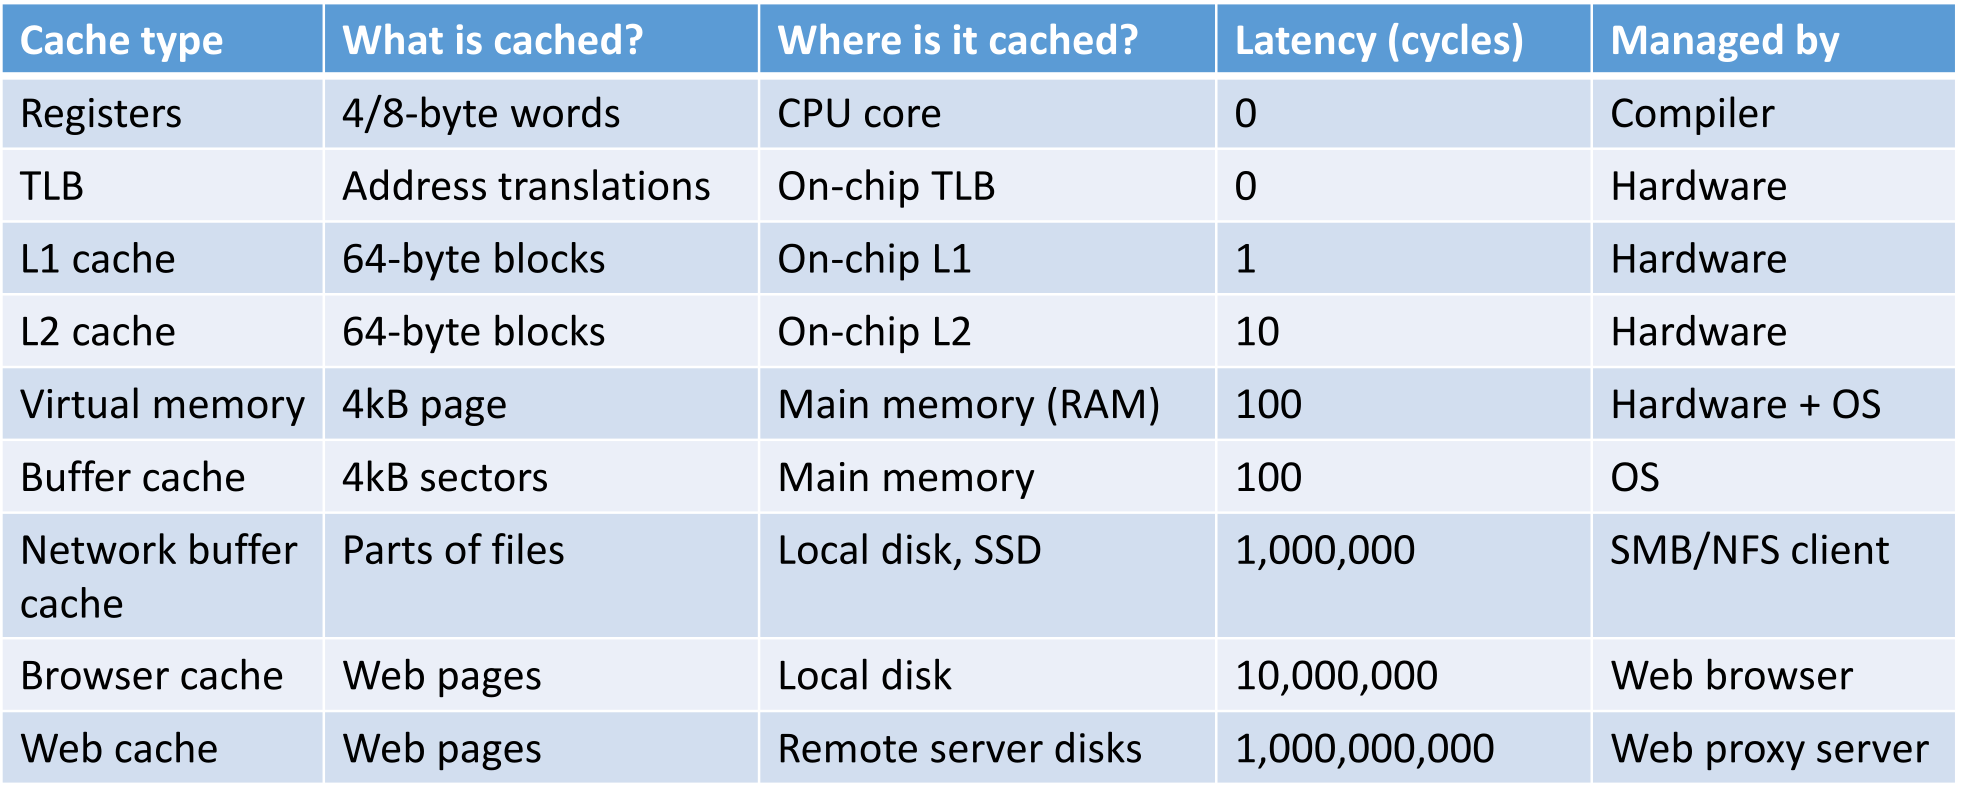
\includegraphics[width=0.8\textwidth]{18_cacheHierarchyTable.png}

Different architectures have different caches. Most CPUs have $3$ different caches and the L1 cache is often split into a instruction and a data cache. This is due to the locality of instruction (if no branch, we access the next instruction) and data (we often need the next data block).

\subsubsection{Cache Writes}

\paragraph{Write Hit}
There are policies on what to do if we write to a block which is also in cache:

\begin{description}
    \item[Write-Through:] Write changes down the hierarchy to memory
        \begin{itemize}
            \item Advantage: Memory is always consistent
            \item Disadvantage: Very slow then we write the same location multiple times
        \end{itemize}
    \item[Write-Back:] Change only value in cache and defer write to memory 
        \begin{itemize}
            \item We need a \textit{dirty} bit which indicates that an entry is different from memory.
            \item Advantage: Higher Performance
            \item Disadvantage: More complex hardware
        \end{itemize}
\end{description}

\paragraph{Write Miss}
These policies describe what do to when we write to a location which is not in memory

\begin{description}
    \item[Write-allocate:] Load block into cache and update the entry only in the cache
        \begin{itemize}
            \item Advantage: Good if there are more writes to this location
            \item Disadvantage: More complex hardware and this may evict existing blocks from cache
            \item Common with write-back caches
        \end{itemize}
    \item[No-Write-Allocate:] Write change to memory
        \begin{itemize}
            \item Advantage: Simpler to implement
            \item Disadvantage: Slower if there are multiple writes to the same location
            \item Common with write-through caches
        \end{itemize}
\end{description}

\paragraph{Other Features}
There are other demission to be made when designing a cache:

\begin{description}
    \item[Unified:] Instructions and data is in the same cache
        \begin{itemize}
            \item Often, L1 is not unified and L2 and L3 caches are unified
        \end{itemize}
    \item[Private vs Shared:] Is the cache exposed to other cores or only a single one
        \begin{itemize}
            \item Often, L1 and L2 are private while L3 is shared
        \end{itemize}
    \item[Inclusive vs Exclusive:] 
        \begin{itemize}
            \item If everything which is is this cache is \textbf{also in all} lower-level caches, it is incisive.
                \begin{itemize}
                    \item Is easier for eviction policy
                \end{itemize}
            \item If anything which is in this cache is \textbf{not in any} lower-level cache, it is exclusive.
            \item Often, only L3 is inclusive and L1 and L2 are exclusive
        \end{itemize}
\end{description}

\paragraph{Software Caches}
Software caches allow for more flexible and complex policies.

\subsubsection{Cache Optimisations}

\paragraph{Principle of Locality}
The reason why caches work, is due to locality. Programms tend to use data and instruction with addresses near or equal to recently used ones.

\begin{description}
    \item[Temporal Locality:] Recently referenced items are likely to be referenced again in the near future.
    \item[Spatial Locality:] Items with nearby addresses tend to be referenced close together in time.
\end{description}

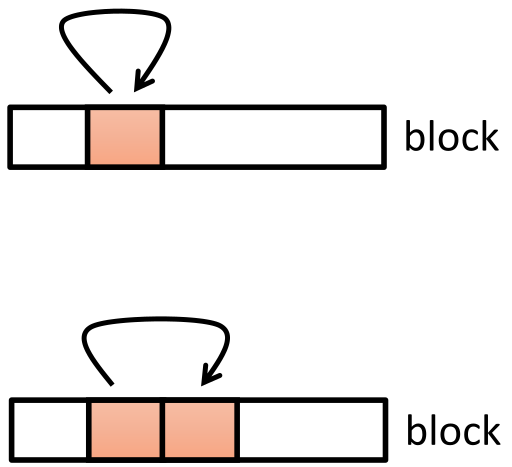
\includegraphics[width=0.8\textwidth]{18_locality.png}

\paragraph{Optimisation for the Memory Hierarchy}
As a programmer, it is important to consider the locality of code. E.g. a linked list is not contiguously in memory. Furthermore, once data is fetched, we should do as much work with if, was we can.

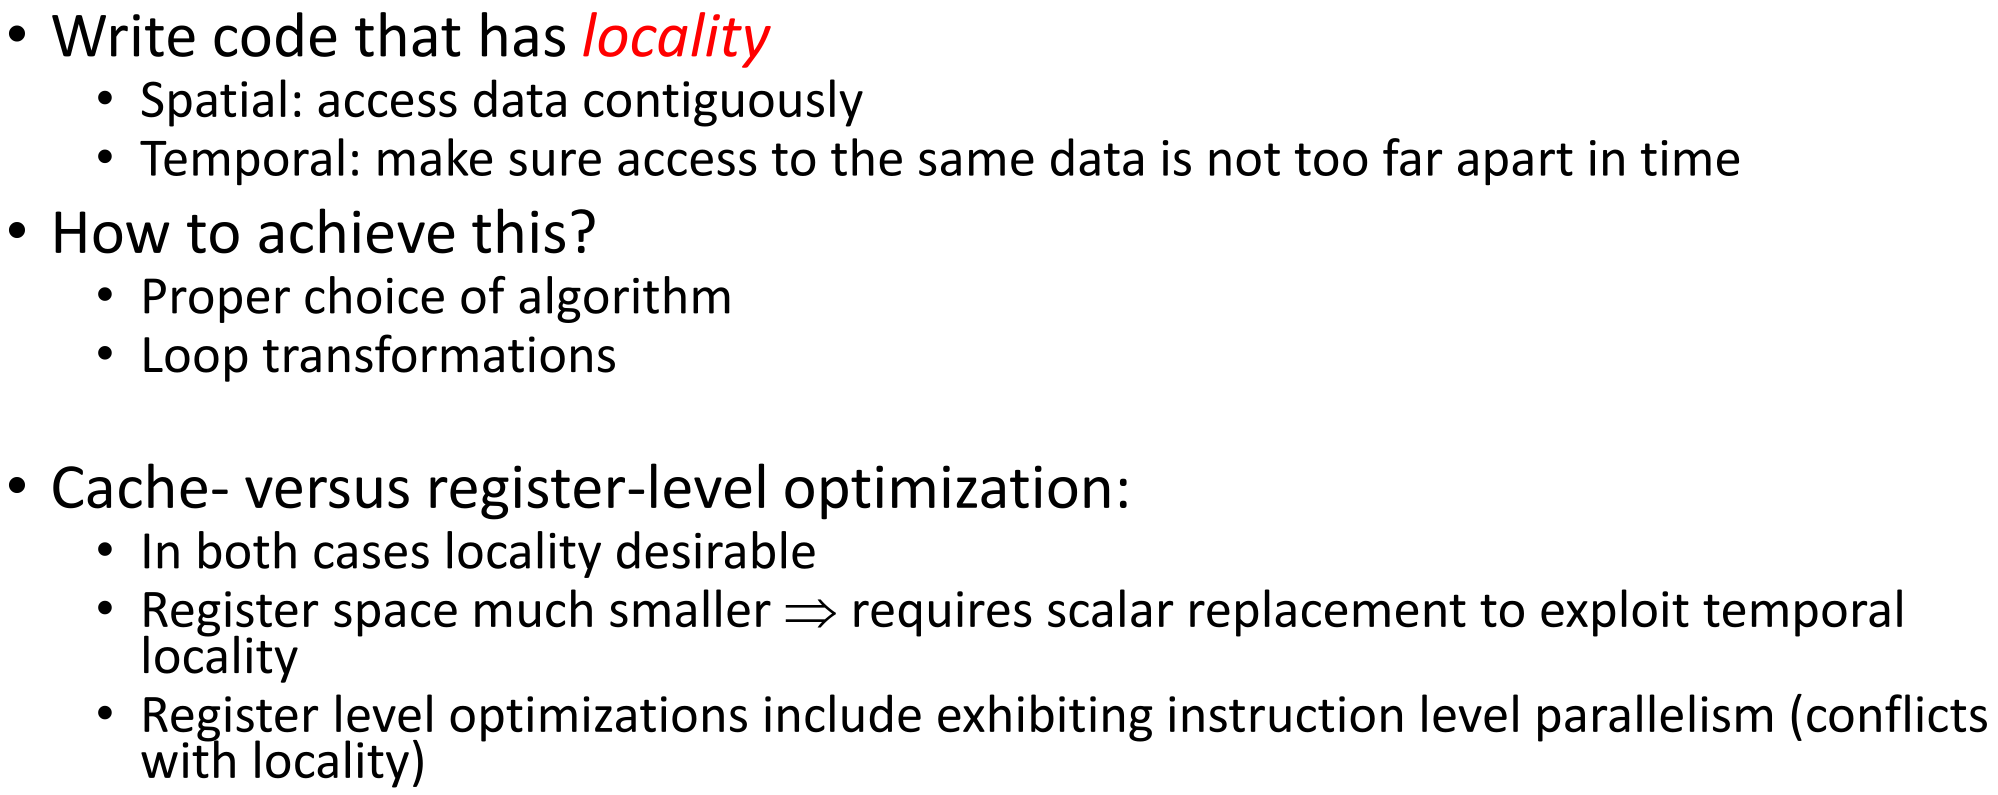
\includegraphics[width=1\textwidth]{18_optimisationMemoryHierarchy.png}

\paragraph{Example: Matrix Multiplication}
Matrix multiplication is a great algorithm do demonstrate usage of locality. And how the performance can be drastically improved when considering locality.

The most trivial implementation is probably:

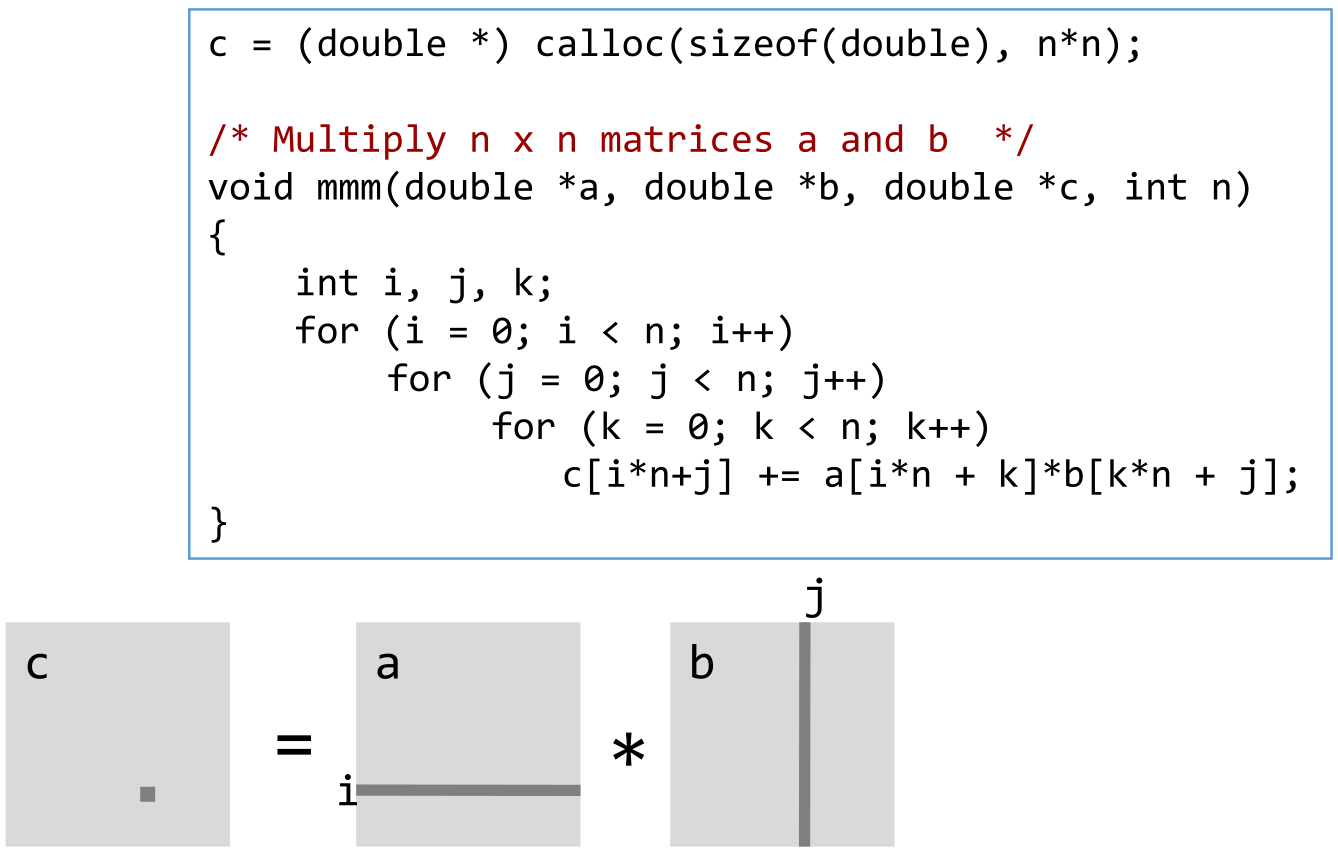
\includegraphics[width=1\textwidth]{18_matrixMultiplication.png}

In order to analyse the cache miss, we assume:
\begin{itemize}
    \item Matrix elements are doubles
    \item Cache block $= 8$ doubles
    \item Cache size $C << n$ (I.e. we cannot load the whole matrix into cache)
\end{itemize}

For the first iteration of the inner loop we have $\frac{n}{8} + n = \frac{9n}{8}$ misses. The first operand are the misses for matrix A, the $n$ misses for operand B.

For the following $n^2$ repetitions we get the same number of misses, thus the total number of misses is $\frac{9n}{8} \cdot n^2 = \frac{9}{8} \cdot n^3$.

When doing block matrix multiplication, we try to make better use of locality by changing the order in which we access elements.

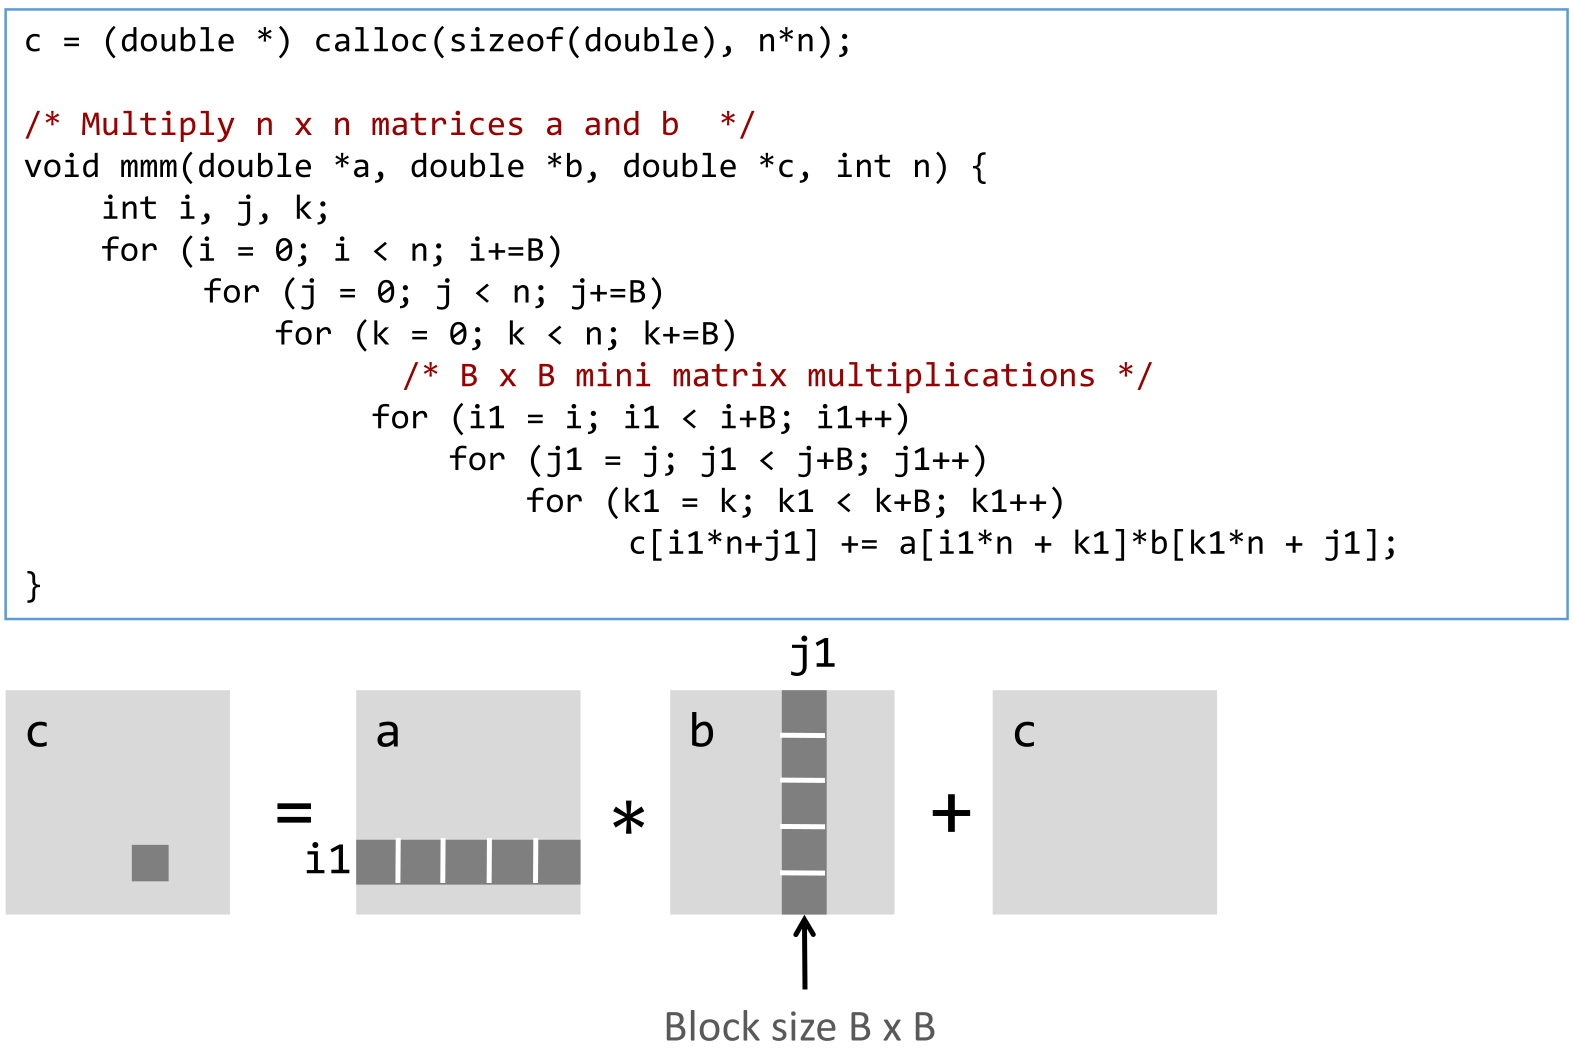
\includegraphics[width=0.8\textwidth]{18_blockMatrixMultiplication.png}

Additionally, to the previous assumptions, we assume that three blocks fit into cache ($3B^2 < C$). So $B$ is a free parameter, but restricted by this assumption.

For one blocks, we have a total of $\frac{B^2}{8}$ misses. The first block iteration we have $\frac{2n}{B} \cdot \frac{b^2}{8} = \frac{nB}{4}$ many misses.

The number of misses for each iteration is equal. Thus, we get a total number of misses of $\frac{nB}{4} \cdot (\frac{n}{B})^2 = \frac{n^3}{4B}$.


The reason of the drastic difference between non-blocking ($\frac{9}{8} \cdot n^3$ and blocking ($\frac{1}{4B} \cdot n^3$ is because matrix multiplication has inherent temporal locality.
